%Template Disclaimer: I used a Latex Template for the general structure of the writeup

\documentclass[11pt,a4paper]{article}

% Encoding, language, fonts
\usepackage[utf8]{inputenc}
\usepackage[T1]{fontenc}
\usepackage[english]{babel}
\usepackage{tikz}
\usepackage{float}
\usetikzlibrary{calc}

% Page layout and header/footer
\usepackage[margin=1in]{geometry}
\usepackage{fancyhdr}
\pagestyle{fancy}
\fancyhf{}
\lhead{Short Title}
\rhead{\thepage}
\chead{}
\renewcommand{\headrulewidth}{0.4pt}

% Math and symbols
\usepackage{amsmath,amssymb,amsthm,mathtools}
\numberwithin{equation}{section}
\usepackage{bm} % bold math symbols
\newcommand{\R}{\mathbb{R}}
\newcommand{\vect}[1]{\bm{#1}}
\newcommand{\deriv}[2]{\frac{\mathrm{d} #1}{\mathrm{d} #2}}
\newcommand{\T}{\mathbf{\Theta}}
\newcommand{\state}{\mathbf{\Psi}}
\newcommand{\X}{\mathbf{X}}
\newcommand{\To}{\mathbb{T}}

% Theorem environments
\newtheorem{theorem}{Theorem}[section]
\newtheorem{lemma}[theorem]{Lemma}
\theoremstyle{definition}
\newtheorem{definition}[theorem]{Definition}
% Assumption theorem style
\newtheoremstyle{assumption} % name
    {6pt}   % Space above
    {6pt}   % Space below
    {\itshape}% Body font
    {0pt}   % Indent amount
    {\bfseries}% Theorem head font
    {.}     % Punctuation after theorem head
    { }     % Space after theorem head
    {}      % Theorem head spec

\theoremstyle{assumption}
\newtheorem{assumption}[theorem]{Assumption}

% Rationale sub-environment to use inside an assumption
\newenvironment{rationale}{%
  \par\vspace{0.5em}
  \noindent\hspace{1em}\begin{minipage}{\dimexpr\linewidth-2em}
  \underline{\textit{Rationale:}} 
}{%
  \end{minipage}
  \par\vspace{0.5em}
}


\usepackage{graphicx}
\usepackage{subcaption}
\graphicspath{{figures/}{results/}}


% Hyperlinks
\usepackage[hidelinks]{hyperref}

% Bibliography (biblatex + biber)
\usepackage[backend=biber,style=alphabetic]{biblatex}
\addbibresource{refs.bib} % create refs.bib beside this file

% Useful utilities
\usepackage{xspace}
\usepackage{enumitem}

% Metadata
\title{Title Goes Here}
\author{Caiman Moreno-Earle \\ California Institute of Technology \\ \texttt{cmorenoe@caltech.com}}
\date{\today}

\begin{document}

\maketitle

\begin{abstract}
% Brief abstract (one paragraph). Replace with actual abstract.
\end{abstract}

\tableofcontents
\bigskip
% \listoffigures
% \listoftables

\section{Introduction}
% Purpose, scope, related work pointers (no actual content here).

\section{Theory / Background}
We begin by establishing the theoretical kinematic dynamics governing the swarm of birds, and then using 
these dynamics to infer the flow of information through the system. Analysis of several videos of swarming shows
that a full swarm may be comprised of several sub-swarms. For the purposes of this paper, we will denote each of these 
sub-swarms as a \textit{component} \cite{swarm_video_youtube}.

\begin{definition}
A \textbf{component} is defined as the tuple $(C, r)$, a set of birds, $C$, such that any bird in the component 
may be reached from any other bird in the component via a sequence of birds, each within radius $r$ of the next.
\end{definition}

\begin{assumption}
    All swarms are composed of a finite number of components. 
    \begin{rationale}
        There exists a finite number of birds in the universe (hopefully) and 
        thus even in the worst case scenario where each bird is its own component, 
        there will still be a finite number of components.
\end{rationale}
\end{assumption}

\begin{assumption}
    The behavior of birds within a component $(C,r)$ is independent of the behavior of birds outside the component.
    \begin{rationale}
        Information and therefore influence may only be transmitted bird 
        to bird within a limited radius, for convienience
        assume $r$ is chosen to be less than or equal to this radius.
    \end{rationale}
\end{assumption}

Under assumptions 2.1 and 2.2 it suffices to analyze the behavior of a single component.
So for now consider a single component $(C,r)$. Let $N=|C|<\infty$ be the number
of birds in the component. 
\begin{definition}
    A \textbf{state} at time $t$ is a vector
    \[
        \Psi(t) = (\theta_1(t), \theta_2(t), \ldots, \theta_N(t), X_1(t), X_2(t), \ldots, X_N(t)) \in \R^{6N},
    \]
    where \(\theta_i(t), X_i(t) \in \mathbb{R}^3\) represent the heading and position of bird \(i\) in space at time $t$ (heading taken to be normalized).
\end{definition}

Let $\Psi_{0}$ be the initial state of the system at time $t=0$. 
The evolution of the system can then be modeled by the following initial value problem
\begin{align}
    \begin{cases}
    \displaystyle \frac{\mathrm{d}\Psi(t)}{\mathrm{d}t} = F(\Psi(t)),\\[6pt]
    \Psi(0) = \Psi_{0}
    \end{cases}
\end{align}

where $F: \R^{6N} \to \R^{6N}$ is a function that encodes interactions between birds in the system.

\begin{assumption}
    $F$ is continuous and differentiable in $\Psi$ on a neighborhood of $\Psi_0$.
    \begin{rationale}
        Being a physical system, between macroscopic objects (birds) we should
        expect the interactions to be continuous and at least $C^1$ smooth.
    \end{rationale}
\end{assumption}


\begin{assumption}
    Under small time scales the relative separations, $\|X_i-X_j\|$, of birds
    in the swarm can be considered constant.
    \begin{rationale}
        Studies have determined that topological properties (i.e. closest neighbors not metric distance of closest neighbors)
        matter more in bird flocking behavior than metric distance, so for small time scales we can assume
        that distances between birds remain constant without affecting end behavior of system
        \cite{ballerini2008interaction}
    \end{rationale} 
\end{assumption}

Looking at assumption 2.5 let us now consider its implications. First 
we can define the separation $N \times N$ matrix $K(t)$, constructed as \(K_{i,j}(t) = \|X_i(t) - X_j(t)\|\):
\begin{equation}
    K(t) = 
    \begin{bmatrix}
    \|X_1(t) - X_1(t)\| & \|X_1(t) - X_2(t)\| & \cdots & \|X_1(t) - X_N(t)\| \\
    \|X_2(t) - X_1(t)\| & \|X_2(t) - X_2(t)\| & \cdots & \|X_2(t) - X_N(t)\| \\
    \vdots & \vdots & \ddots & \vdots \\
    \|X_N(t) - X_1(t)\| & \|X_N(t) - X_2(t)\| & \cdots & \|X_N(t) - X_N(t)\|
    \end{bmatrix}
\end{equation}

Under a small time scale $t\in(t_0,t_0+\delta)$, we can consider $K(t)$ to be constant matrix by assumption 2.5, which we
will denote $K$. The final simplification we make is to furhter restrict positions $X_i(t)$ to be in a lattice structure, 
to simplfiy analysis and neiborhood computations.

\begin{assumption}
    Under a small time scale, the positions $X_i(t)$ of birds in the component are fixed on a lattice structure in $\R^3$.
    \begin{rationale}
        From assumption 2.5 we know that under a small time scale the relative separations of birds remain constant,
        now also referring to \cite{ballerini2008interaction} we know that birds
        focus more on topological neighbors rather than metric neighbors, so since 
        for this model we are more concerned about turning and heading information rather than exact positions
        we can assume a lattice structure.
    \end{rationale}
\end{assumption}


Now for a small time scale equation (2.1) can be rewritten as a system of first oder ODEs
\begin{equation}
    \begin{cases}
    \displaystyle \frac{\mathrm{d}\theta_i(t)}{\mathrm{d}t} = f_i(\theta_1(t), \theta_2(t), \ldots, \theta_N(t); K), & i=1,2,\ldots,N,\\[6pt]
    \theta_i(0) = \theta_{i,0}, & i=1,2,\ldots,N,
    \end{cases}
\end{equation}

\begin{theorem}[Existence and Uniqueness of Solutions to (2.3)]\label{thm:existence_uniqueness}
Let $F$ be as defined in (2.1), then there exists a unique local solution corresponding to the IVP (2.3) 
\end{theorem}

\begin{proof}
From assumption 2.5 we know that $F$ is differentiable and therefore by MVT locally lipschitz in $\Psi$ on a neighborhood of $\Psi_0$.
Now it follows that for each $f_i$ in (2.3), $f_i$ is also locally lipschitz in $\theta_j$ on a neighborhood of $\theta_{j,0}$. therefore
by Picard–Lindelöf theorem there exist unique solutions (2.3) for small time scales.
\end{proof}

The remainder of this paper will focus on analyzing the solutions to this system of equations, 
with a second order variation of this system being considered in section [TBD].

\section{Swarm on a Sphere Analysis}
% Additional theory, lemmas, proofs.
As discussed in the introduction the two main methods we will use to analyze the first-order system (2.3), are the 
Swarm on a Sphere (SOS) model and the Generalize Ising Model. First we will examine this system through the SOS approach.
To build up to SOS we first introduce the Kuramoto model. The Kuramoto model is a model in mathematical physics to describe
 a system of synchronizing oscillators. that take the from 
\begin{equation}
    \begin{cases}
            \frac{d\psi_i}{dt}=\omega_i + \frac1N \sum_{j=1}^N R_{ij} sin(\psi_j-\psi_i)\\
            \psi_i(0)=\psi_{i,0}
    \end{cases}
\end{equation}
Where $\psi_i$ represents the phase of the $i$th oscillator, $\omega_i$ its natural frequency, and $R_{ij}$ the coupling strength between oscillators $i$ and $j$.
\\
While I would have loved to use Kuramoto to model the heading in (2.3), the main 
limitation is that $\psi_i(t)\in \R^2$, while accurately modeling (2.3) requires $\theta_i(t)\in \R^3$ (again assumed normalized).

The generalization of this model to $d-dim$ is the the Swarm on a Sphere (SOS) model \cite{SOS}, which models
coupled oscillators on $\mathbb{R}^d$. Where in our context $d=2$ and the oscillators represent the heading of each bird in the swarm.
SOS is given by the follwing 
\begin{equation}
        \frac{dx_i}{dt}=\sum_{j=1}^N R_{ij}(x_j-\langle x_j,x_i\rangle x_i)\\ 
\end{equation}

Where $x_i\in \mathbb{R}^d$ is the unit vector of bird $i$ in the swarm, and $R_{ij}$ the interaction strength between birds $i$ and $j$.
We get that $\theta_i = x_i$. and thus \(f_i\) is given by the RHS of (3.2). Before analyzing (3.2) analytically, 
we first numerically experiment to determine key parameters that affect the behavior of the system, then we
analyze the system to determine stability and long term behavior of solutions. 

\subsection{Computational Experiments}
\subsubsection{Implementation}
The goal of the computational experimetns was to numerically determine 2 key parameters that affect the behavior,
namely the intial allginment and the interaction matrix $R$.
\begin{definition}
    The \textbf{initial alignment} of a component $(C,r)$ is defined as 
    \[
        A = \frac{1}{N} \left\| \sum_{i=1}^N \theta_{i,0} \right\| \in [0,1].
    \]
    Where $A=1$ represents perfect initial allignment (all birds facing the same direction) and $A=0$ represents
     initial disallignment (birds in random directions).
\end{definition}

To accomplish this I wrote a python simulation that numerically solves (3.2) on a 3D lattice using scip's IVP solver.
The simulation works by approximating a component $(C,r)$ on a $X\times Y\times Z$ 3D lattice with edge length $r$ between lattice points, and 
$N=X \times Y \times Z$. Each vertex represents a bird with an associated heading (unit vector in $\R^3$). 
\\

To intialzie the simulation takes in the size of the flock $(X,Y,Z)$, an initial alignment $A$ which 
is what determiens the distribution of initial headings of the birds, and an intteraction matrix $R$.
Since from \cite{ballerini2008interaction} we know that interactions are based off of topological neighbors,
the interaction matrix $R$ is constructed based off of \textbf{order}, and \textbf{weight}.
\begin{figure}
    \centering
    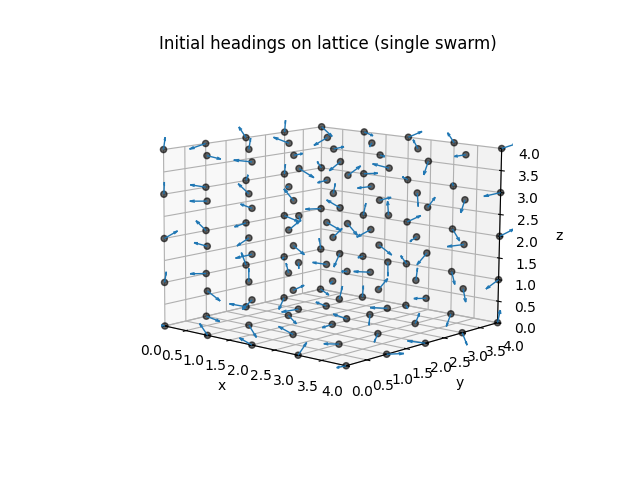
\includegraphics[width=0.5\textwidth]{lattice_headings.png}
    \caption{Visualization of Initial Heading Allginents on Lattice}
\end{figure}

\begin{definition}
    The \textbf{order} of the interaction matrix $R$ on a lattice $L$, is defined as the maximum
    lattice "hops" two birds may be and still interact. (i.e. order 1 means birds only interact with direct lattice neighbors, order 2 neighbors of neighbors and so on).
\end{definition}

\begin{definition}
    The \textbf{weight} of the interaction matrix $R$ on a lattice $L$, is defined as the strength of interaction
    between birds that are at the maximum order of interaction.
\end{definition}

\begin{figure}[h]
    \centering
    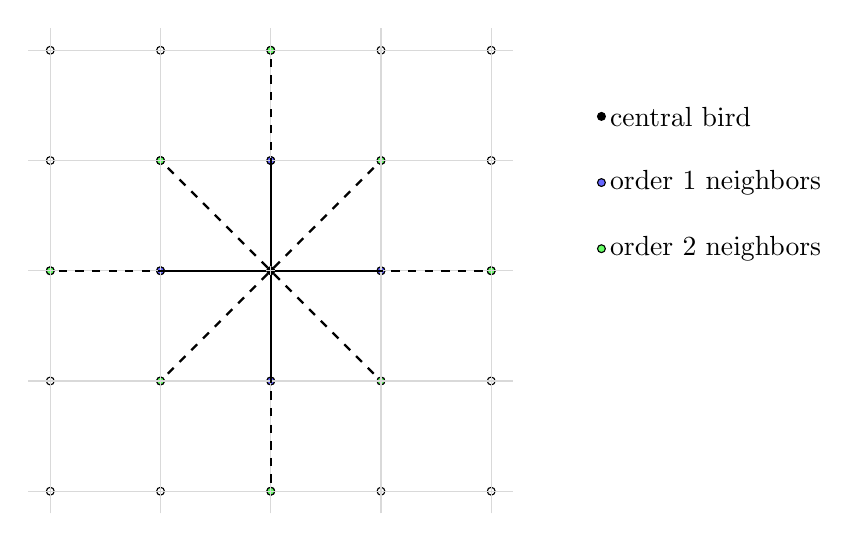
\begin{tikzpicture}[scale=1.4, every node/.style={circle, draw, inner sep=1pt}]
        % Lattice points (5x5)
        \foreach \x in {-2,-1,0,1,2} {
            \foreach \y in {-2,-1,0,1,2} {
                \node[fill=white] (n\x\y) at (\x,\y) {};
            }
        }

        % Central bird
        \node[fill=black] (center) at (0,0) {};

        % Order 1 neighbors (distance 1 in L1 metric)
        \node[fill=blue!60] (n10) at (1,0) {};
        \node[fill=blue!60] (n-10) at (-1,0) {};
        \node[fill=blue!60] (n01) at (0,1) {};
        \node[fill=blue!60] (n0-1) at (0,-1) {};

        % Order 2 neighbors (within 2 lattice hops but not order 1)
        % Horizontal/vertical at distance 2
        \node[fill=green!60] (n20)  at (2,0) {};
        \node[fill=green!60] (n-20) at (-2,0) {};
        \node[fill=green!60] (n02)  at (0,2) {};
        \node[fill=green!60] (n0-2) at (0,-2) {};
        % Diagonals at distance 2 (1+1)
        \node[fill=green!60] (n11)   at (1,1) {};
        \node[fill=green!60] (n1-1)  at (1,-1) {};
        \node[fill=green!60] (n-11)  at (-1,1) {};
        \node[fill=green!60] (n-1-1) at (-1,-1) {};

        % Draw grid in light gray (optional)
        \foreach \x in {-2,-1,0,1,2} {
            \draw[gray!30] (\x,-2.2) -- (\x,2.2);
        }
        \foreach \y in {-2,-1,0,1,2} {
            \draw[gray!30] (-2.2,\y) -- (2.2,\y);
        }

        % Interaction edges:
        % Order 1 edges (thick)
        \draw[thick] (center) -- (n10);
        \draw[thick] (center) -- (n-10);
        \draw[thick] (center) -- (n01);
        \draw[thick] (center) -- (n0-1);

        % Order 2 edges (thick, dashed to indicate weaker interaction)
        \foreach \nodeName in {n20,n-20,n02,n0-2,n11,n1-1,n-11,n-1-1} {
            \draw[thick,dashed] (center) -- (\nodeName);
        }

        % Legend
        \node[fill=black, label=right:{central bird}] at (3.0, 1.4) {};
        \node[fill=blue!60, label=right:{order 1 neighbors}] at (3.0, 0.8) {};
        \node[fill=green!60, label=right:{order 2 neighbors}] at (3.0, 0.2) {};
    \end{tikzpicture}
    \caption{Order 1 and 2 interaction on a 2D lattice (AI Disclaimer: I used chatGPT to generate this tikz drawing)}
    \label{fig:order2-2d}
\end{figure}

As it is obvious that if all else is kept equal, a higher order will lead to quicker swarm alignment, to
accurately determine the appropriate order I give every bird a constant "attention", $At$ such that 
\begin{equation}
    At = \sum_{j=1}^N R_{ij}, \quad \forall i=1,2,\ldots,N.
\end{equation}   
This means that as order increases, the weight must decrease simulating that it is harder
for brids to pay attention to more birds at any given time. I finally ran several simulation 
over a sweep of initial alignments, orders, and weights, over a variety 
of flock sizes to determine which values created realistic flocking behavior.

\subsubsection{Computational Results}
\begin{figure}[ht]
    \centering
    % Top row
    \begin{subfigure}{0.45\textwidth}
        \centering
        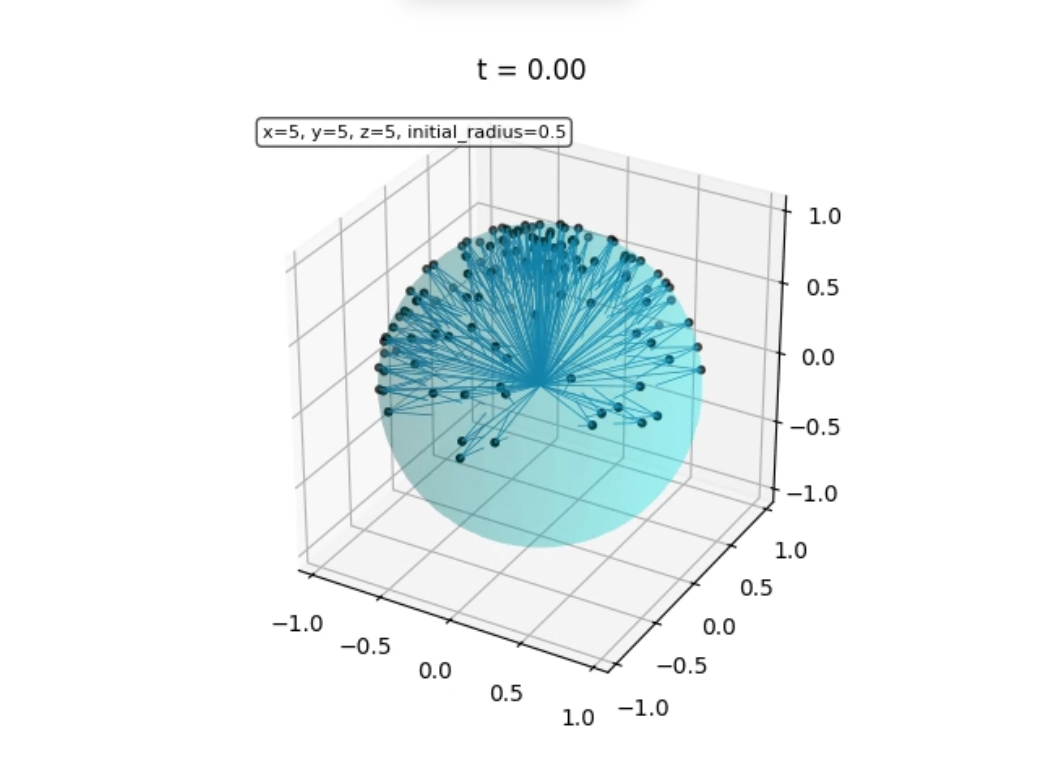
\includegraphics[width=\textwidth]{initial_heading_1s.png}
        \caption{Intial Headings with $A=0.5$.}
        \label{fig:order1-A02}
    \end{subfigure}
    \hfill
    \begin{subfigure}{0.45\textwidth}
        \centering
        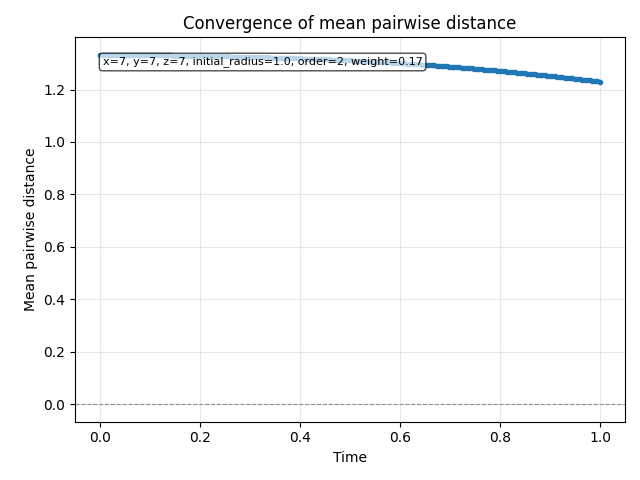
\includegraphics[width=\textwidth]{bad_conv_1.png}
        \caption{Allignment Convergence for Order 1, initial alignment $A=1$.}
        \label{fig:order1-A08}
    \end{subfigure}

    \vspace{0.5em}

    % Bottom row
    \begin{subfigure}{0.45\textwidth}
        \centering
        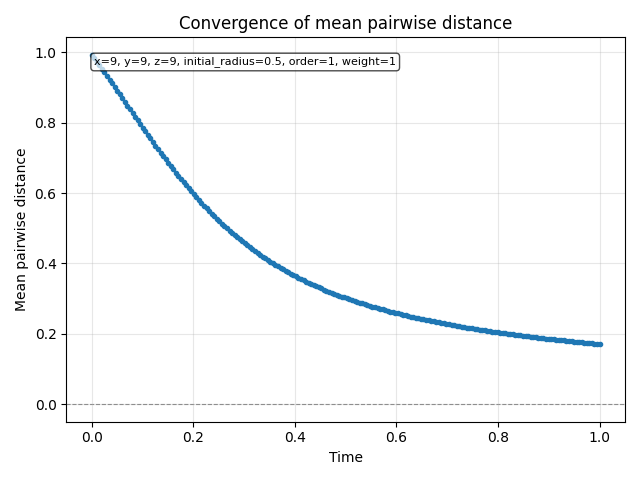
\includegraphics[width=\textwidth]{good_conv_1.png}
        \caption{Allignment Convergence for Order 1, initial alignment $A=0.5$.}
        \label{fig:order2-A02}
    \end{subfigure}
    \hfill
    \begin{subfigure}{0.45\textwidth}
        \centering
        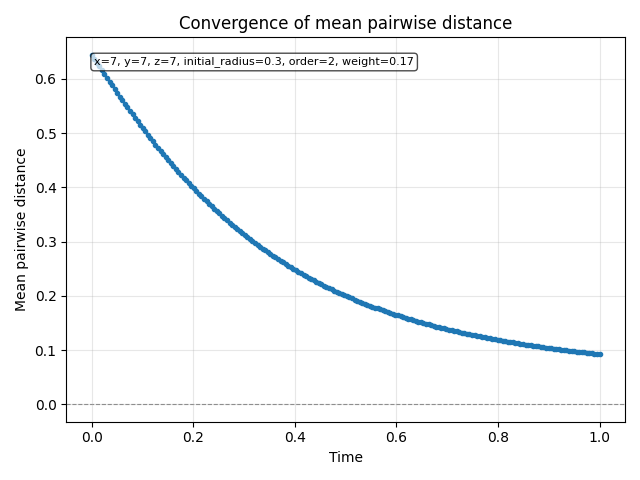
\includegraphics[width=\textwidth]{mid_conv_1.png}
        \caption{Allignment Convergence for Order 2, initial alignment $A=0.3$.}
        \label{fig:order2-A08}
    \end{subfigure}

    \caption{Comparison of swarm behavior for different interaction orders and initial alignments.}
    \label{fig:order-A-grid}
\end{figure}
%
% TO DO LATER 
%    -introduce the graphs and such
%    -explain the parameters found
%    -talk about cool behavior with interacting swarms
%
\begin{figure}[H]
    \centering
    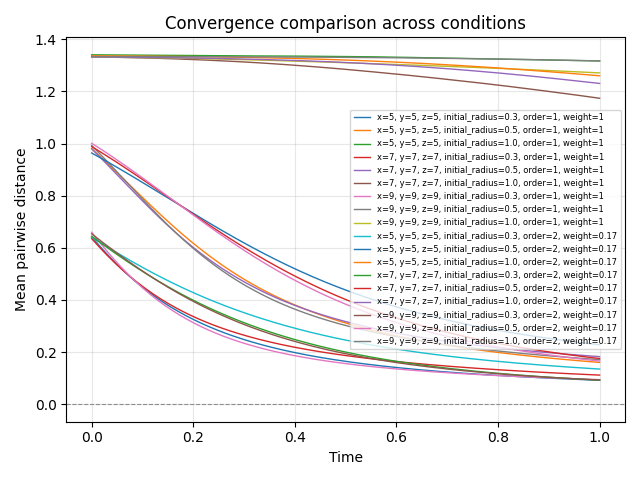
\includegraphics[width=0.7\textwidth]{sos_convergence_overlay.png}
    \caption{Order 1 simulation result.}
    \label{fig:overlay}
\end{figure}
From the results of the experiments, and primarily figure \ref{fig:overlay}, we conclude
two main results. First, higher order interactions converge slower than order 1 interactions, 
and second, there appears to be a critical alignment value $A_c >0.5$ such that for $A<A_c$ swarms converge to allignment, and for $A>A_c$ swarms diverge to disallignment, or at the very 
least converge too slowly to be realistic. This leads us to assume that 
real world flocking behavior is best modeled by order 1 interactions with initial alignments below $A_c$.
\\

While order 1 interactions seem physcially intuitive, as you wouldn't expect brids to be tracking huge numbers of negihbors at a time, the results regarding intial alligment beg several questions.
While it makes sense that after an intial period of congregation birds in a component
would generally be partially alligned, this begs the question of how would flocks intially form given that intial alignment is likely 0. To anwser this question I turned into \textbf{swarm collision}.
\\

\subsubsection{Swarm Collisions}
While playing around with the simulation I noticed an interesting behavior that if two 
swarms with low total alignment, had subgroups that were highly alligned, then the solution 
would rapidly converge to allignment. This led me to experiment wiht the idea of \textbf{swarm collision}

\begin{definition}
    A \textbf{swarm collision} is defined as when two alligned components $(C_1,r_1)$ and $(C_2,r_2)$ physically overlap in
    position space such that their interactions can be modeled as a single component $(C,r)$ with $C=C_1\cup C_2$ and $r=\max(r_1,r_2)$, 
    and the lattice represneting the system made with birds from $C_1$ and $C_2$ are randomly mixed. (ex. figure \ref{fig:swarm-collision}).
\end{definition}
\begin{figure}[H]
    \centering
    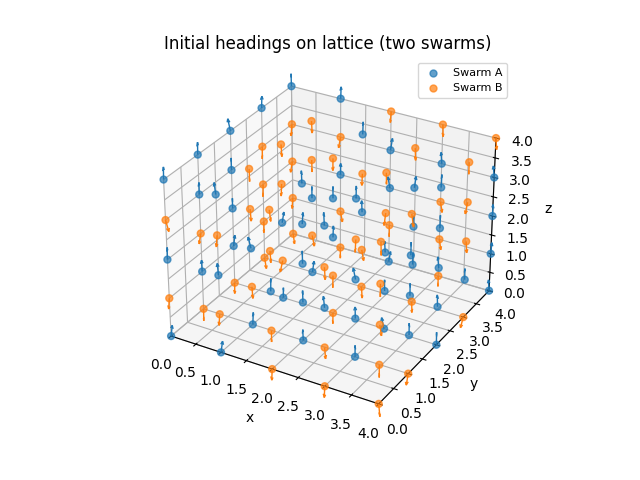
\includegraphics[width=0.7\textwidth]{swarm_collisions_lattice.png}
    \caption{Intial Headings between two colliding swarms}
    \label{fig:swarm-collision}
\end{figure}

I simulated these collisions and compared their convergence to that of a single swarm with no
intial allignment. The results are presented in figure \ref{fig:2s} and \ref{fig:collision-overlay}. 
You can see in figure \ref{fig:collision-overlay} that despite having near identical intial headings
the two swarm collision converges significantly faster than the random initial allignment case.

\begin{figure}[ht]
    \centering
    % Top row
    \begin{subfigure}{0.45\textwidth}
        \centering
        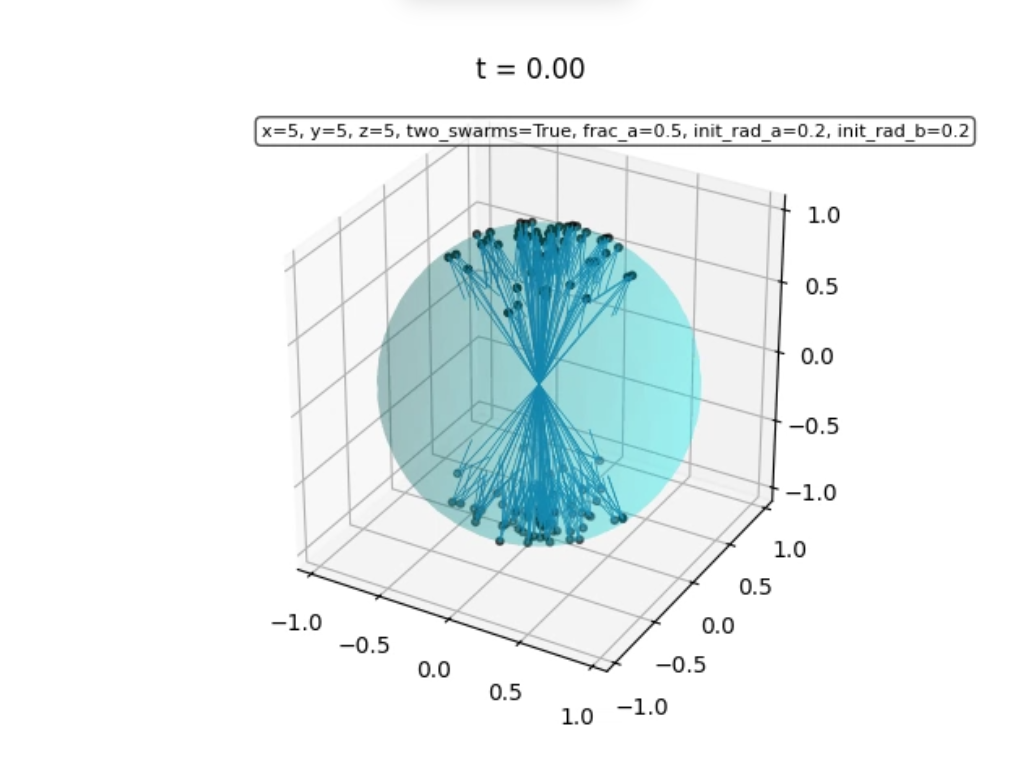
\includegraphics[width=\textwidth]{initial_heading_2s.png}
        \caption{Swarm Collision $t=0$}
        \label{fig:ih_2s1}
    \end{subfigure}
    \hfill
    \begin{subfigure}{0.45\textwidth}
        \centering
        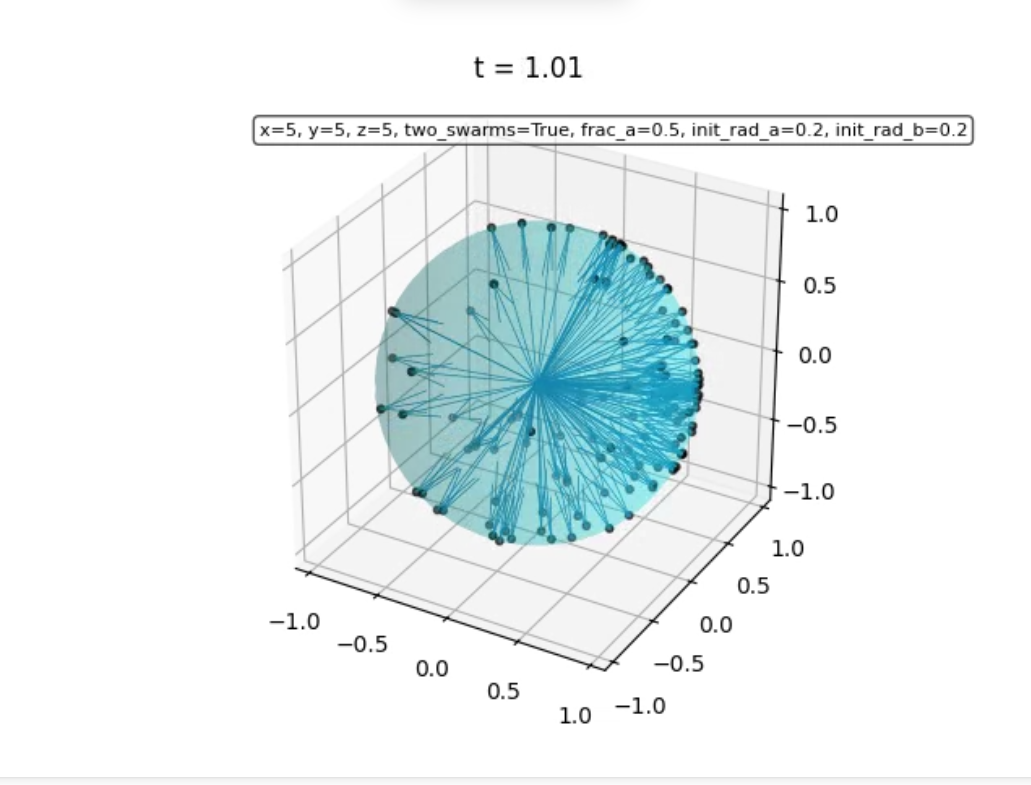
\includegraphics[width=\textwidth]{ih_2s2.png}
        \caption{Swarm Collision $t=1$}
        \label{fig:ih_2s2}
    \end{subfigure}

    \vspace{0.5em}

    % Bottom row
    \begin{subfigure}{0.45\textwidth}
        \centering
        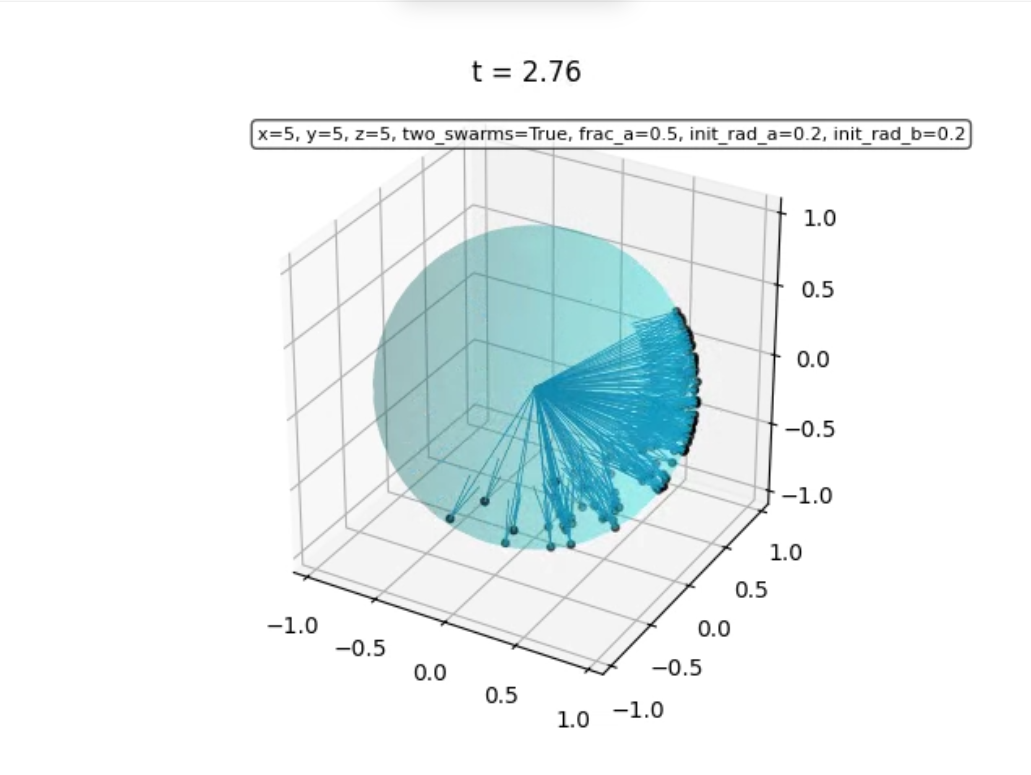
\includegraphics[width=\textwidth]{ih_2s3.png}
        \caption{Swarm Collision $t=2.5$}
        \label{fig:ih_2s3}
    \end{subfigure}
    \hfill
    \begin{subfigure}{0.45\textwidth}
        \centering
        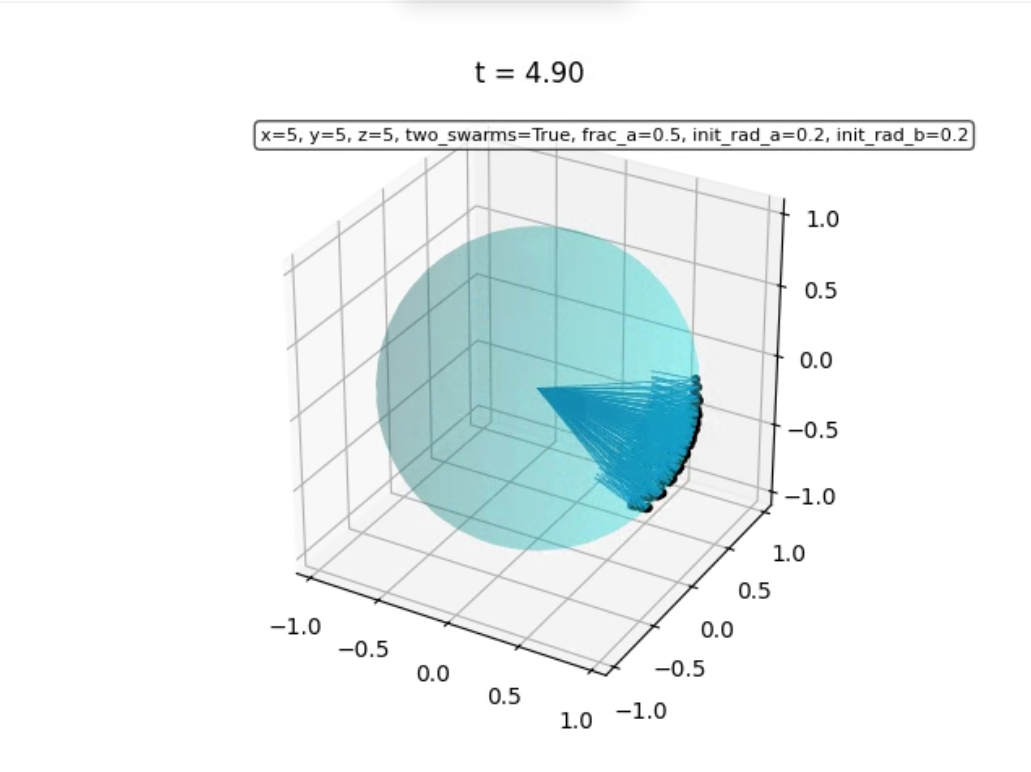
\includegraphics[width=\textwidth]{ih_2s4.png}
        \caption{Swarm Collision $t=5$}
        \label{fig:ih_2s4}
    \end{subfigure}

    \caption{Evolution of Two Swarm Collision}
    \label{fig:2s}
\end{figure}
\begin{figure}[H]
    \centering
    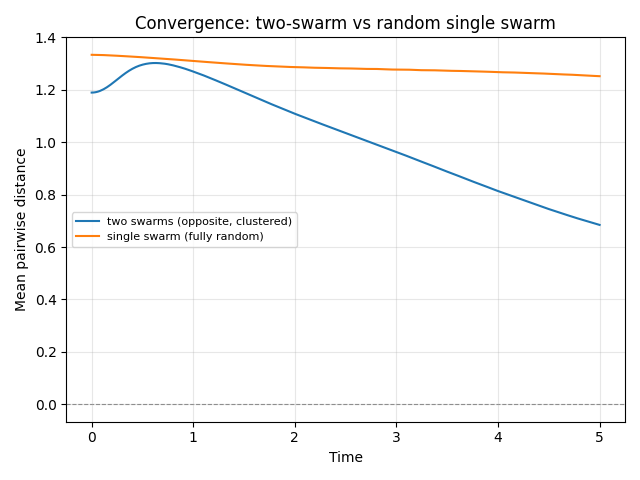
\includegraphics[width=0.7\textwidth]{sos_two_swarm_vs_random.png}
    \caption{Two Swarm Collision vs Random Initial Alignment}
    \label{fig:collision-overlay}
\end{figure}

\subsection{Analytical Results}
From setions (3.1.1) and (3.1.2) we fully define $F$ in (2.1) as the RHS of (3.2) with an order 1 interaction matrix $R$.
Now we can analyze the stability of solutions to (3.2) under these conditions.

First let us determine the asymptotic behavior of solutions to (3.2). 
\begin{theorem}[Solutions to (3.2) are Asymptotically Stable]\label{thm:asymptotic_stability}
\end{theorem}
\begin{proof}
    Let $\theta_i(t)$ be a solution to (3.2) with interaction matrix

Let $\T=(\theta_1, \theta_2, \ldots, \theta_n)$ Define a Lyapunov function
\begin{align}
    V_i(\T) &= \frac12 \sum_{j=1}^N R_{ij}(1-\langle \theta_j, \theta_i \rangle)\\
    V(\T) &= \sum_{i=1}^N V_i(\T)
\end{align}
Since $\|\theta_i\|=1 \ \forall i$ and from (3.1) we have that $R_{ij}\geq 0 \ \forall i,j$
we have that $V(\T)\geq 0 \ \forall \T$, and since $R$ is overlapping (neighborhood of each bird intersects with 6 other birds in 3D) $V(\T)=0$ iff $\theta_i=\theta_j \ \forall i,j$.

Now we calculate $\dot V(\T)$ along solutions to (3.2)
\begin{align}
    \dot V(\T) &= \frac{\partial V}{\partial t} + 
    \frac{\partial V}{\partial \T}{f} \\
    &= 0 + \sum_{i=1}^N \sum_{j=1}^N \frac{\partial V_i}{\partial \theta_j} \cdot f_j \\
    &= \sum_{i=1}^N \langle \frac{\partial V}{\partial \theta_i}, \dot \theta_i \rangle
\end{align}
Now note that since the interaction matrix $R$ is symmetric we have that
\begin{align}
    \frac{\partial V}{\partial \theta_i} &= \sum_{j=1}^N \frac{\partial V_j}{\partial \theta_i} \\
    &= -\sum_{j=1}^N R_{ji} \theta_j
\end{align}
Noting that from (3.2) we have that
\begin{align}
    \dot \theta_i = f_i &= \sum_{j=1}^N R_{ij}\theta_j - \sum_{j=1}^N \langle \theta_j, \theta_i \rangle \theta_i\\
    &= -\frac{\partial V}{\partial \theta_i} + \langle \frac{\partial V}{\partial \theta_i}, \theta_i \rangle \theta_i
\end{align}
Letting $P_i = -\sum_{j=1}^N R_{ji} = \frac{\partial V}{\partial \theta_i}$ we can substitute in to 
(3.8) to get 
\begin{align}
\dot V(\T) &=  - \sum_{i=1}^N \langle P_i, P_i - \langle P_i, \theta_i \rangle \theta_i \rangle \\
&= - \sum_{i=1}^N \left( \|P_i\|^2 - \langle P_i, \theta_i \rangle^2 \right)
\end{align}
Finally realize that 
\begin{align}
    \|f_i\|^2 &= \|P_i - \langle P_i, \theta_i \rangle \theta_i\|^2 \\
    &= \|P_i\|^2 - 2\langle P_i, \theta_i \rangle^2 + \langle P_i, \theta_i \rangle^2\|\theta_i\|^2\\
    &= \|P_i\|^2 - \langle P_i, \theta_i \rangle^2
\end{align}
Where (3.17) holds since our headings live on the unit sphere. Therefore substituting (3.17) into (3.15) we get
\begin{align}
    \dot V(\T) &= - \sum_{i=1}^N \|f_i\|^2\\
    &\leq 0
\end{align}
Finally by again noting that $R$  is overlapping and all non-zero entires equal we have that $\dot V(\T)=0$ iff $\theta_i=\theta_j \ \forall i,j$.
Thus since  $\theta_i=\theta_j \ \forall i,j$ is also our condition for $V(\T)=0$ we have that by Lyapunov's direct method that
all solutions to (3.2) are globaly uniformly asymptotically stable.  \cite{lyapunov_stability_theory} 
\qedhere
\end{proof}





\subsection{Conclusion from SOS Analysis}
From the computational experiments we can conclude a few key points regarding the formation and behavior of 
bird flocks. First, individual birds in a flock likely only monitor the headings of their order 1 ($6$ in 3D) neighbors when 
turning. Next, there exists a critical intial alignemnt $A_c$ such that flocks with $A<A_c$ will rapidly 
converge to allignment when flying. Finally the results of section (3.1.3) conclusion leads us to the final (and in my opinion most interesting) conclusion
that large bird flocks form from the collision of smaller, already aligned sub-swarms, building the size of the flock over time. 
tu
\\

Finally from theorem \ref{thm:asymptotic_stability} we have that under the SOS model (3.2) all swarms will eventually converge to allignment, 
regardless of intial alignment. This reinforces the convergence result from the computational experinces, and also clarrifies
that $A_c$ is not a rigoroud cirtical point rather points with lower initial allignment simply converge many orders faster than those with higher initial allignment.


\section{Heisenberg Model Analysis}
While section 3 anwsered some key questions regarding flock behavior, primarily 
flock formation interaction order and stability, the question of the speed of information
flow and response to a predator attack remains. 

I first thought of using the Heisenberg model when I looked at figure \ref{fig:swarm-collision} and saw that
the headings of the birds in a lattice resembeled the spins of particles in an antiferromagnetic material 
(a material where the lowest energy states are when spins are anti-parrell), and when they reach 
allignment they resembeled the spins of particles in a ferromagnetic material (a material where the lowest energy states are when spins are parrell).
\\

And this is where the Heisenberg model comes in. The Heisenberg model is a statistical mechanics model
that models the spins of particles in a lattice ferromagnetic or antiferromagnetic material. The hamiltonian for such a system is given by
\begin{equation}
    H =  -J\sum_{\langle i,j \rangle} S_i \cdot S_j - \mu \sum_i B \cdot S_i
\end{equation}
Where $S_i$ is the spin vector of particle $i$, $J$ is the interaction strength between direct neighboring spins $\langle i,j \rangle$ , $\mu$ is the magnetic moment, and $B$ is an external magnetic field \cite{heisenberg_model_pires}.
If $J>0$ the lowest energy states are those such that all spins are parallel so the material is ferromagentic. For our puproses 
we use say our system is "ferromagnetic" because we want the flock to tend to a state where all brids are alligned in the same direction.

Solutions to this system are usually analytically intractable, so we introudce a final simplifcation of the system.
\begin{assumption}
    For the purposes of modeling the speed of information flow, it suffices to consider heading to be a discrete variable in $\{-1,1\}$.
    \begin{rationale}
    While in sections 2 and 3 heading was modeled as a continuous variable in this section we are less concerned about \textit{how} birds
    allign and more concerned about how \textit{fast} they allign, and making this simplfication allows us to simplify to a model that is analytically tractable. 
\end{rationale}
\end{assumption}












\section{Discussion}

\section{Conclusion}

\section*{AI Disclaimer}
ChatGPT was used for very specific parts of this
project. The following are the ONLY parts which AI was 
in any way involved with:
\begin{itemize}
    \item The Tikz drawing in figure \ref{fig:order2-2d} was generated with the help of ChatGPT.
    
    \item The formating to get the subfigures in figure \ref{fig:order-A-grid} and \ref{fig:2s} side by side was 
    assisted by ChatGPT.

    \item As noted in the header note of the SOS.py, AI was used to 
    help write certain plotting and visualization functions, however all computational experiments, testing,
    and analysis were written SOLEY by me
    \item An online template and AI were used at the very beginning
    of this project to format a blank latex document with formatting, 
    but absolutely no content was populated during this phase
\end{itemize}

\appendix
\section{Supplementary material}

\printbibliography

\end{document}